\chapter{相关技术介绍}
\section{Spark平台介绍}
Apache Spark\cite{zaharia2010spark}是为了快速计算而设计出来的集群计算技术。它基于Hadoop MapReduce技术,并且扩展了Hadoop MapReduce模型来有效地进行更多类型的计算,包括交互式查询以及流处理。Spark最主要的特性是内存集群计算技术,将数据保持在内存而不序列化到硬盘上大大提高了计算速度。

Spark最早是由UC Berkeley的Matei Zaharia在2009年作为Hadoop的一个子项目进行开发的。它在2010年基于BSD证书开源并在2013年捐献给了Apache Software Foundation(ASF)。从2014年的二月起,Spark已经成为了ASF中的顶级项目之一。Apache Spark官网将Spark定义为大规模数据处理的一个快速、通用的引擎。

Spark有如下主要特性:
\begin{itemize}
    \item \textbf{速度快}。如果数据全部在内存中,Spark平台上的计算能比Hadoop MapReduce快100倍以上,如果将数据序列化到硬盘上,则能快10倍以上。
    \item \textbf{便于使用}。Spark支持Java/Scala/Python/R四种语言的API,提供了超过80多种高度抽象的操作来使得编写并行程序更加容易,并且提供了Scala,Python和R的交互式Shell用以快速熟悉并验证原型程序。
    \item \textbf{通用性}。Spark联合了SQL、streaming和complex analytics。Spark由SQL and Dataframes, MLLib for machine learning\cite{meng2015mllib}, GraphX和Spark Streaming驱动。我们可以在同一个程序中无缝地联合使用这么多库。
    \item \textbf{随处运行}。Spark可以运行在Hadoop、Mesos、独立模式,还可以方便地部署到现有的商业云上。Spark可以访问包括HDFS、Cassandra、HBase和S3等在内的多种数据源。我们可以在独立集群模式下或者EC2或者Hadoop YARN或者Apache Mesos下运行Spark,访问位于HDFS、Cassandra、HBase、Hive、Tachyon和任何Hadoop数据源。
\end{itemize}

Spark有如下四部分主要组成:
\begin{figure}[ht]
\centering
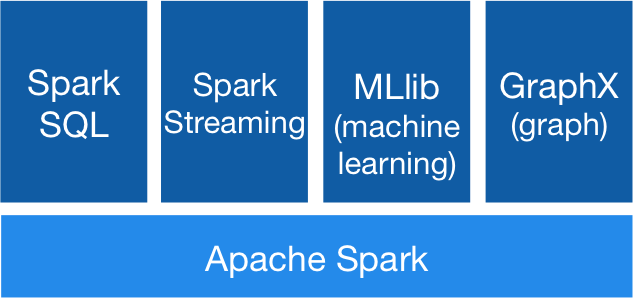
\includegraphics[width=10cm]{spark-stack}
\caption{Spark Stack}
\end{figure}
\begin{itemize}
    \item \textbf{Spark SQL}。Spark SQL使得你可以通过Java、Python、R、Scala语言在Spark程序中使用SQL或者熟悉的DataFrame API来查询结构化数据。并且DataFrames和SQL提供了一种通用的方式来访问多种不同的数据源,包括Hive, Avro, Parquet, ORC, JSON和JDBC。我们甚至可以使用对数据使用连接(join)操作。Spark SQL完全兼容Hive的操作,我们可以对于已有的数据运行未经修改的Hive查询。通过JDBC和ODBC,我们可以使用标准的数据库连接方式。
    \item \textbf{Spark Streaming}。Spark Streaming提供了Apache Spark语言级整合的API来进行流处理,我们可以像编写批处理任务的代码一样来编写流任务。支持Java、Scala、Python。容错性较高,开箱支持从lost work和operator state中恢复。Spark中不同部分整合性较好,我们可以把流处理和批处理以及交互式请求方便地结合起来。
    \item \textbf{Spark MLlib}。Spark中方便使用的机器学习库,MLlib可以和Python中的Numpy库进行交互,使用任何Hadoop数据源(HDFS, HBase或者本地文件),这使得MLlib很容易插入Hadoop workflow中。在性能上,Spark中的高质量算法,比MapReduce快100倍。Spark非常方便部署,我们可以在Hadoop 2集群上不预装任何东西的情况下运行Spark和MLlib。
    \item \textbf{GraphX}。灵活性非常好,我们可以在collections和graphs之间无缝整合,GraphX在单个系统中统一了ETL,解释分析,迭代图计算。我们可以把同一份数据视为graphs或者collections,采用Spark中transform或者join graphs操作。在性能上,与其他专门的图处理系统相比Spark是最快的。在算法数量上,Spark拥有相当多的图算法实现,包括PageRand, Connected components, label propagations, SVD++, Strongly connected components, Triangle count等。
\end{itemize}

\subsection{Spark内部结构}
Spark中内部情况如图\ref{fig:clusterOverview}。
\begin{figure}[ht]
\centering
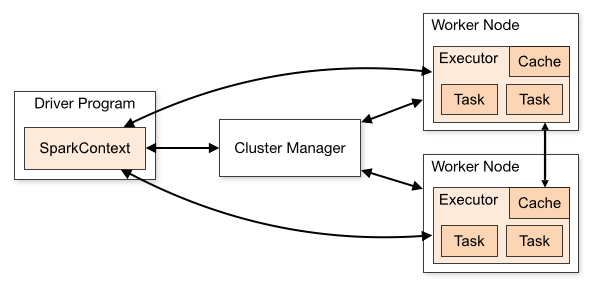
\includegraphics[width=10cm]{cluster-overview}
\caption{cluster overview}\label{fig:clusterOverview}
\end{figure}
一个Spark集群,由初始化了SparkContext的驱动程序,和许许多多个工作节点组成。
我们把程序提交到Spark Driver上,由cluster manager来进行任务调度,实际的计算任务几乎都落在Spark的工作节点上。由于任务调度的关系,驱动程序和工作节点最好能够在同一个局域网下,不然因为网络延迟以及带宽的缘故,花在网络等待的时间可能较长,会影响到计算的时长。
\subsection{Spark基本编程模型}
Spark中最基本的数据类型是弹性分布式数据集RDD( Resilient Distributed Dataset)\cite{zaharia2012resilient}。它可以通过读取Hadoop InputFormat或者通过其他RDD Transform得到。在Spark中由两种最基本的操作transform和action,可以认为分别是Map和Reduce的扩展。

下面介绍一下我们的算法中用到的一些Spark提供的变换和操作。如表\ref{spark:transform}和表\ref{spark:action}。
\begin{table}[htbp]
\centering
\caption{Spark中的transformation操作}\label{spark:transform}
\begin{tabular}{|p{5cm}|p{10cm}|}
\hline
map(func)	& 对每个元素使用func操作之后返回新的RDD。\\ \hline
filter(func)	& 过滤func操作结果为假的元素,返回新的RDD。 \\ \hline
flatMap(func)	& 与map相似,但是每个输入元素映射到0或多个输出元素。 \\   \hline
sample(withReplacement, fraction, seed) &	使用给定的随机种子,对输入的数据进行给定比例的采样。 \\ \hline
union(otherDataset)	& 返回输入数据与参数联合的新RDD。 \\   \hline
intersection(otherDataset) &	返回数据数据与参数交集的新RDD。\\ \hline
distinct([numTasks]))	& 返回输入数据中不同元素的新RDD。\\ \hline
groupByKey([numTasks])	& 对数据集(K ,V)对进行操作,返回(K, Iterable<V>)对。\\ \hline
reduceByKey(func, [numTasks]) & 当在(K, V)对上调用的时候,返回(K, V)对数据集。值V必须满足类型(V, V)=>V,然后用func函数进行聚合得到。\\ \hline
sortByKey([ascending], [numTasks])	 & 当K是可排序的,在(K, V)对数据集上调用该函数的时候,返回ascending指定的升序或者逆序排列的(K, V)数据集对。\\ \hline
join(otherDataset, [numTasks]) &	 当在类型为(K, V)和(K, W)的数据集上调用的时候,返回(K, (V, M))的数据集对。此外还有leftOuterJoin/rightOuterJoin/LeftOuterJoin。 \\ \hline
cogroup(otherDataset, [numTasks])	& 在数据类型(K, V) 和(K, W)上进行调用的时候, 返回(K, (Iterable<V>, Iterable<W>))数据集对。\\ \hline
cartesian(otherDataset)	 & 当在数据类型T和U上进行调用时,返回所有的(T, U)对。\\ \hline
\end{tabular}
\end{table}

\begin{table}[htbp]
\centering
\caption{spark中的action操作} \label{spark:action}
\begin{tabular}{|p{5cm}|p{10cm}|}
    \hline
    reduce(func) & 对数据集中的元素使用func函数(输入两个元素,输出一个元素)进行聚合。func函数需要符合结合律和交换律以防在并行计算中出错。\\     \hline
    collect() & 把数据集中的所有元素作为数组返回到驱动程序中。通常在其他操作返回一个较小的数据集后比较有用。\\ \hline
    count() &  返回数据集中元素的个数。\\ \hline
    first() &  返回数据集中的第一个元素。\\ \hline
    take(n) & 返回包含数据集中前n个元素的数组。\\ \hline
    takeSample(withReplacement, num, [seed]) & 返回数据集中随机采样后的数组。\\ \hline
    takeOrdered(n, [ordering]) & 使用自然顺序或者自定义的比较器来返回数据集中的前n个元素。\\ \hline
    saveAsTextFile(path) & 将数据集中的元素写到本地文件系统、HDFS或者其他支持Hadoop的文件系统的指定目录中,每个元素使用toString方法后作为文本的一行。\\ \hline
    countByKey() & 只对(K, V)类型的RDD数据有效. 返回对每个Key进行计数后的(K, Int)的hashmap。\\ \hline
    foreach(func) & 对数据集中的每一个元素应用func函数。\\ \hline
    \hline
\end{tabular}
\end{table}

通常来说,传递给Spark操作(例如Map或Reduce)的函数是在工作节点上运行的。函数内的所有变量在所有节点上都是一份独立的拷贝。在远程工作节点上对于这些变量的修改不会反馈到驱动程序中。在工作节点上,支持通用的可读写的共享变量是低效的。虽然如此,Spark提供了两种有限的共享变量:broadcast variables和accumulators。Broadcast variables允许我们在每台机器上保持一个只读的变量,而不用随着任务下发变量。Accumulators是符合交换律的只能“添加”的变量,在Spark可以用来实现计数器或者求和等操作。

\section{推荐系统介绍}
推荐系统在现在的场景中越来越重要,由于信息的爆炸式增加,互联网上的商品数量也在不断的增加,但是用户能够浏览的信息和商品都是有限的,如何让用户浏览他们需要的东西成为商品/服务提供者所面临的一个问题,这引起了人们对于推荐系统的研究。推荐系统最早是由美国明尼苏达大学的小组进行研究的,目前针对推荐系统的研究较为广泛,推荐系统的应用也较为普遍。在电商行业,推荐系统的重要性更是尤为突出,以Amazon为例,如图\ref{fig:amazon}中,Amazon给购买某产品的用户推荐其他购买该产品的用户也购买了的产品,Amazon的Web界面中处处有着推荐系统的应用。
\begin{figure}[ht]
\centering
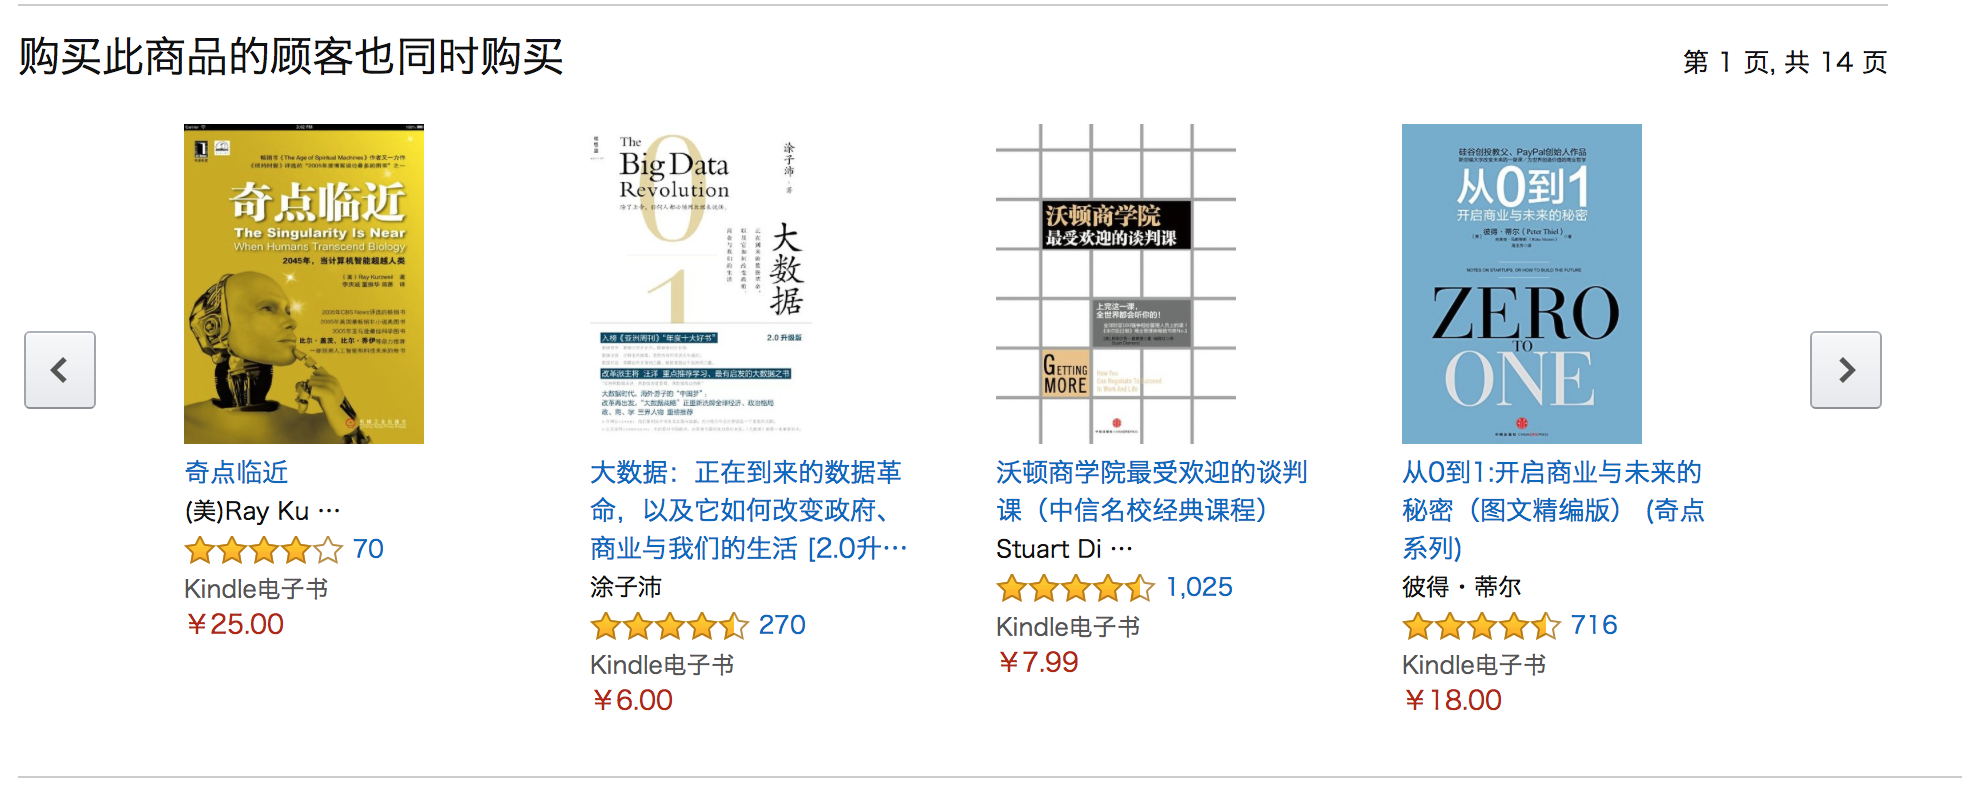
\includegraphics[width=10cm]{amazon}
\caption{Amazon推荐}\label{fig:amazon}
\end{figure}

目前的推荐系统主要可以分为个性化推荐系统与非个性化推荐系统。个性化会根据针对不同用户推荐不同的数据,而非个性化推荐系统考虑的因素没有用户相关的要素。除了基于用户评分的推荐算法,推荐系统还有很多变种,比如基于用户显式评分的推荐系统,基于用户隐式评分的推荐系统,基于信任关系的推荐系统。在推荐系统中也很很多值得研究的问题,比如冷启动问题,如何防止恶意用户攻击推荐系统等。

\subsection{算法总览}
在目前的非个性化推荐系统中,主要考虑是物品的热度。实现方法是对每个物品,用户可以进行投票赞成(up vote),也可以投票反对(down vote),点赞数较多的就可以排在比较靠前的位置。对于需要考虑时间因素的新闻推荐,会综合考虑点赞数和已经发布的时长两个因素,比如在知名的reddit网站,推荐算法有如下的数学表示,其中$A$代表某篇新闻的发布时间,$B$代表过去的某个固定时间点,$t_s$代表他们时间的时间差。
$$ t_s = A - B $$
$U$代表点赞数,$D$代表反对数。
$$x = U - D$$
$y \in \{-1, 0, 1\}$代表了$x$的符号。
$$ y = \begin{cases}
    1 & if\ x > 0 \\
    0 & if\ x = 0 \\
    -1 & if\ x < 0
\end{cases}$$
$z$代表$x$和$1$绝对值的最大值。
$$z = \begin{cases}
\lvert x \rvert  &  if\  \lvert x \rvert \geq 1 \\
1 & if\  \lvert x \rvert < 1
 \end{cases}
$$
最终我们得到评分函数如下公式\ref{eq:reddit},反对时间越晚,用户点赞数$-$反对数越大,分数越高,越靠前:
\begin{equation}\label{eq:reddit}
f(t_s, y, z) = \log_{10}z + \frac{yt_s}{45000}    
\end{equation}
reddit的非个性化推荐系统是较为成功的推荐系统之一,并且系统开销很小。

对于个性化推荐算法推荐算法,主要有我们如下介绍的基于内容过滤和协同过滤两大类,我们将在接下来的章节详细介绍这一部分。

\subsection{基于内容过滤的推荐算法}
基于内容过滤的推荐算法,是根据一个用户消费的商品与其他的商品的相似性来进行推荐。而商品之间的相似性是通过商品的自身属性来计算,不依赖于用户对于商品的评分,适合于在能够获取商品较多的信息下使用。使用基于内容过滤算法的推荐系统,能够避免对于商品的冷启动问题。而基于内容的过滤算法的关键在于对描述商品的信息的选取,通常情况下我们会使用商品的标签(tags)来表示一个商品,标签的添加可以通过人工录入或者机器学习的方式来进行录入。每个标签可以视为一个维度,这样我们可以将一个商品表示成依赖标签的一个向量,通过计算两个向量之间的相似性,我们可以得出商品之间的相关性。我们需要注意的几个问题有,商品之间的标签可能是近义标签,所以需要注意标签的选取。

举例如表\ref{tab:contentFiltering},表中相应的位为0代表没有这个标签,为1则代表有这个属性。
\begin{table*}[htbp]
    \centering
    \caption{以电影为例对基于内容的过滤进行举例}\label{tab:contentFiltering}
    \begin{tabular}{|c|c|c|c|}
        \hline
        电影 & 爱情 & 动作 & 科幻 \\ \hline
        星球大战 & 0 & 1 & 1 \\ \hline
        阿凡达 & 0 & 1 & 1 \\ \hline
        泰坦尼克号 & 1 & 0 & 0 \\ \hline
    \end{tabular}
\end{table*}
对于《阿凡达》和《星球大战》来说,他们在使用三个标签标示的维度下,完全一样,而相对应的《泰坦尼克号》则拥有完全互补的标签,当我们制定了相似性计算规则之后,我们可以认为星球大战和阿凡达更为相似,有理由给喜欢星球大战的用户推荐阿凡达而不是泰坦尼克号。

\subsection{基于协同过滤的推荐算法}
基于协同过滤算法实现的推荐系统不依赖于商品本身的属性信息,仅仅需要收集用户对于商品的评分就可以计算出应该给用户推荐哪些商品,这对于无法收集或者收集商品信息不全的应用场景较为有用。算法基本输入如下,我们有一个用户-商品的评分矩阵如表\ref{tab:ratingmatrix},我们利用用户已经评分过的商品,来计算用户对于未评分的矩阵的期望评分,对用户推荐用户预期评分较高的产品。协同过滤具体可分为两大类算法,基于邻域的推荐算法和基于矩阵分解的隐式因子模型,在下面章节中进行详细介绍。
    \begin{table*}[htbp]
    \centering
    \caption{用户评分矩阵}\label{tab:ratingmatrix}
    \begin{tabular}{|c|c|c|c|c|}
        \hline
        & 物品1 & 物品2 & 物品3 & 物品4 \\ \hline
        用户1 & 2& ? & 3 & 4\\ \hline
        用户2 & ? &4 &  4 & 5\\ \hline
        用户3 & 5 & ?& 2 & ? \\ \hline
    \end{tabular}
    \end{table*}
    
\subsection{基于邻域的推荐算法}
\subsubsection{相似关系}
基于邻域的推荐算法最重要的方法就是描述相似关系,对于物品的相似性的定义关系到计算时的权重分配,使用不同的相似性计量标准会带来有一定差异的相似性结果。常用的相似性计量有很多算法,我们整理如下,当我们计算两个向量$u$和$v$的相似性时,我们可以遵循如下统一的流程对多种相似性计算公式进行计算,首先进行预处理preprocess,预处理后进行标准化norm,最后在套用similarity公式进行计算。如下表\ref{tab:contentFiltering}。
\begin{table}[htbp]
\centering
\caption{相似性关系一览表} \label{tab:similarity}
\begin{tabular}{|c|c|c|c|}
    \hline
    measure & preprocess & norm & similarity\\
    \hline
    Cosine & $\frac{v}{\lVert v \rVert}$ & - & $dot_{ij}$ \\
    \hline
    Pearson correlation & $\frac{v - \bar{v}}{\lVert v - \bar{v} \rVert}$ & - & $dot_{ij}$ \\
    \hline
    Euclidean distance & - & $\hat{v}^2$ & $\sqrt{n_i - 2 \cdot dot_{ij} + n_j}$ \\
    \hline
    Common neighbors & $bin(v)$ & - &$dot_{ij}$ \\
    \hline
    Jaccard coefficient & $bin(v)$  & $\lVert \hat{v} \rVert $  & $ \frac{dot_{ij}}{n_i + n_j - dot_{ij}}$ \\
    \hline
    Manhattan distance & $bin(v)$ & $\lVert \hat{v} \rVert$ & $ n_i + n_j - 2 \cdot dot_{ij}$ \\
    \hline
    Pointwise Mutual Information & $bin(v)$ & $\lVert \hat{v} \rVert$ & $ \frac{dot_{ij}}{\lvert U \rvert} \log \frac{dot_{ij}}{n_in_j} $ \\
    \hline
    Salton IDF & $bin(v)$ & $\lVert \hat{v} \rVert$ & $ \frac{\lvert U \rvert \cdot dot_{ij}}{n_jn_j^2}(-\log\frac{n_i}{U})$ \\
    \hline
    Log Odds & $bin(v)$ & $\lVert \hat{v} \rVert$ & $ \log \frac{ \frac{ \lvert U \rvert \cdot dot_{ij} }{ n_jn_{j}^{2} } }{1 - \frac{ \lvert U \rvert \cdot dot_{ij}}{n_in_{j}^{2}}}$ \\
    \hline
    Loglikehood radio & $bin(v)$ & $\lVert \hat{v} \rVert$ &
    $\!\begin{aligned}[t]
    & 2\cdot (H(dot_{ij}, n_j - dot_{ij}, n_j - dot_{ij}, \\
    &\lvert U \rvert - n_i - n_j + dot_{ij}) \\
    &    - H(n_j, \lvert U \rvert - n_j) - H(n_i, \lvert U \rvert - n_i))
    \end{aligned} $\\
    \hline
\end{tabular}
\note{表的相似性关系及其数学表示}
\end{table}
基于领域的推荐算法可以通过使用用户-用户之间的相似关系,物品与物品之间的相似关系细分为两类。

\subsubsection{用户与用户之间的相似关系}
每个用户和其他用户之间的相似关系可以通过该用户给消费过的物品评分来计算。我们可以认为每个物品都是一个维度,每个用户都是在高维空间的一个向量,用户对商品的评分是对于用户的度量,通常我们使用余弦角度公式\ref{eqn:cos}来计算相似性。
    \begin{equation}\label{eqn:cos}
       similarity(\vec{A}, \vec{B}) = cosine(\vec{A}, \vec{B}) = \frac{\vec{A} \cdot \vec{B}}{\lVert\vec{A}\rVert\ast\lVert\vec{B}\rVert}
    \end{equation}
    我们可以通过计算两个用户共同评分过的的物品的评分组成的向量之间的夹角,通过夹角的大小我们来评估用户之间的相似性。当夹角超过90度的时候,我们认为用户之间存在负相关性。这种负相关性不需要出现在我们的用户的邻居中,需要剔除掉。如果两个用户共同评价的商品只有一个,向量蜕化到标量,相似性计算必然为1,这种情况需要去掉。传统的串行算法如算法\ref{alg:useruserrecseq}。

 \begin{algorithm}
        \caption{基于用户相似性关系的串行Top-N推荐算法}\label{alg:useruserrecseq}
        \begin{algorithmic}[1] %每行显示行号
            \Require \\
            \begin{itemize}
                \item $M$, 用户-物品评分矩阵。每个$M_{u,i}$元素代表代表一个评分或者为空。
                \item $u$,我们希望为其进行计算的用户。
                \item $n$,希望推荐的商品数目。
                \item $Sim(u, v)$,计算两个向量之间的的相似性的函数
                \item $WeightedSums(u, S)$计算对一个给定的用户计算某个商品推荐得分的函数
                \item $TopNRecommendations(R_u, n)$,用来给排序出Top-N高评分的商品的函数。
            \end{itemize}
            \Ensure $R_u(n)$,给用户u推荐的Top-N商品。

        
            \For{$user\ v \in M$}
                \If{ $v \neq u$}
                    \State $S_{u, v} \leftarrow Sim(u, v)$
                \EndIf 
                \For{$item\ i \in M$}
                    \If{$u\ did\ not\ interac\t with\ i$}
                        \State $R_u \leftarrow WeightedSums(u, i, S_{u, v})$
                    \EndIf
                \EndFor
            \EndFor 
            \State $R_u(n) = TopNRecommendatiions(R_u, n)$
        \end{algorithmic}
    \end{algorithm}

\subsubsection{物品与物品之间的相似关系}
基于物品-物品之间的相似性关系的计算,在算法上与基于用户-用户的的推荐算法十分相似,如果将用户评分矩阵转置之后再输入到算法中,那么后续步骤就是一样的,这里就不详细展开说明了。需要注意的是,就是如果存在两个物品只有一个用户评分的话,向量蜕化到标量,那么他们之间的相似性必然为1,我们在计算相似性的时候,要去掉这种情况。

\subsection{隐式因子模型}
隐式因子分解模型通常使用矩阵分解来来完成,我们使用
ALS(Alternating Least Square) 最小交替二乘法\cite{Zachariah:2012hh}算法来进行矩阵分解的计算。我们把行数为用户数$m$,列数为物品数$n$的$m \times n$矩阵分解成为两个$m \times f$和$ f \times n$的矩阵。我们把分解出的因子矩阵认为是描述了物品和用户特征的矩阵,与在基于内容的推荐中的可以显式解释的矩阵做出区分,称之为隐式因子。
我们有用户$u$和$i$如下公式
$$
Q_{ui} = \begin{cases}
r  & \text{if user u rate item i} \\
0 & \text{if user u did not rate item i}
\end{cases}
$$
$r$是评分的真实数据。如果我们有$m$个用户$n$和物品,我们希望从评分矩阵中学习出代表物品和用户特征的的矩阵。学习出可以代表用户的因子向量,可以让我们在特征空间中表示这个用户。学习出来能够表示物品的因子列向量,同样可以在特征空间中表示这个物品。对于物品分解出的矩阵$Y \in \mathbb{R}^{f \times n}$(每部电影都是一列)和用户的因子矩阵$X \in \mathbb{R}^{m \times f}$(每个用户是一个行向量)。由于我们有两个未知的变量需要计算。我们采用一种使用正则化的交替最小二乘法来进行求解。通过这样,我们先使用$X$来求解$Y$,再使用$Y$来$X$。通过足够次数的迭代,我们可以到达一个收敛点,此时矩阵$X$和$Y$都在迭代中不再改变,或者改变极小。虽然如此,在数据中有一个小问题。我们没有完整的用户数据,也没有完整的物品数据,这也是我们我们希望设计实现推荐系统的本意。因此我们在更新过程中没有获取评分的的电影进行惩罚。这样我们仅仅依赖于用户已经评分过的电影的评分数据,而不用依赖于在推荐系统中还没有评分的数据。我们定义了一个权重$w_{ui}$如下
$$w_{ui} = \begin{cases}
0 &\text{if  } q_{ui} = 0 \\
1 & \text{ else} 
\end{cases}$$

现在我们需要定义我们的优化目标,定义损失函数(loss function)如下。
$$J(x_u) = (q_u - x_u Y) W_u (q_u - x_u Y)^T + \lambda x_u x_u^T$$
$$J(y_i) = (q_i - X y_i) W_i (q_i - X y_i)^T + \lambda y_i y_i^T$$
我们致力于优化这个函数。注意到我们加入了正则化系数来避免对于数据的过拟合(overfiting)。这个损失函数是有解的,我们可以不需要利用梯度下降的方法,而是直接求解来完成。解如下
$$x_u = (Y W_u Y^T + \lambda I)^{-1} Y W_u q_u$$
$$y_i = (X^T Wi X + \lambda I)^{-1} X^T W_i q_i$$
注意到这里$x_{u_1}$和$x_{u_2}$之间并无关系,这就使得我们可以在不同的机器上并行计算这些值。
$W_u \in \mathbb{R}^{n\times n}$ 和
$W_i \in \mathbb{R}^{m\times m}$都是对角矩阵。对于正则化系数的选择我们可以通过交叉验证来完成。

\subsection{内容过滤与协同过滤之间的比较}
协同过滤相比内容过滤的优势如下
\begin{enumerate}
    \item 不需要了解商品的内容
    \item 可以适应用户一直在变化的兴趣
    \item 可解释性更好(基于邻域的推荐算法)
    \item 推荐的多样性更好(ALS)
\end{enumerate}
协同过滤相比内容过滤的劣势如下
\begin{enumerate}
    \item 用户评分的矩阵十分稀疏带来了计算上的困难。
    \item 隐私泄露问题。
    \item 可能存在针对性的恶意评分,会影响到给其他用户的推荐。
\end{enumerate}
